\documentclass[12pt,a4paper]{article}
\usepackage[T1]{fontenc}
\usepackage{amsmath,amssymb,mathrsfs,tikz,times,pifont}
\usepackage{enumitem}
\usepackage{multicol}
\usepackage{lmodern}
\usetikzlibrary{trees}
\newcommand\circitem[1]{%
\tikz[baseline=(char.base)]{
\node[circle,draw=gray, fill=red!55,
minimum size=1.2em,inner sep=0] (char) {#1};}}
\newcommand\boxitem[1]{%
\tikz[baseline=(char.base)]{
\node[fill=cyan,
minimum size=1.2em,inner sep=0] (char) {#1};}}
\setlist[enumerate,1]{label=\protect\circitem{\arabic*}}
\setlist[enumerate,2]{label=\protect\boxitem{\alph*}}
%%%::::::by chnini ameur :::::::%%%
\everymath{\displaystyle}
\usepackage[left=1cm,right=1cm,top=1cm,bottom=1.7cm]{geometry}
\usepackage[colorlinks=true, linkcolor=blue, urlcolor=blue, citecolor=blue]{hyperref}
\usepackage{array,multirow}
\usepackage[most]{tcolorbox}
\usepackage{varwidth}
\usepackage{float} %pour utiliser l'option [H] qui force l'image à apparaître exactement à l'endroit où elle est placée dans le code.
\tcbuselibrary{skins,hooks}
\usetikzlibrary{patterns}
\usetikzlibrary{calc}
%%%::::::by chnini ameur :::::::%%%
\newtcolorbox{exa}[2][]{enhanced,breakable,before skip=2mm,after skip=5mm,
colback=yellow!20!white,colframe=black!20!blue,boxrule=0.5mm,
attach boxed title to top left ={xshift=0.6cm,yshift*=1mm-\tcboxedtitleheight},
fonttitle=\bfseries,
title={#2},#1,
% varwidth boxed title*=-3cm,
boxed title style={frame code={
\path[fill=tcbcolback!30!black]
([yshift=-1mm,xshift=-1mm]frame.north west)
arc[start angle=0,end angle=180,radius=1mm]
([yshift=-1mm,xshift=1mm]frame.north east)
arc[start angle=180,end angle=0,radius=1mm];
\path[left color=tcbcolback!60!black,right color = tcbcolback!60!black,
middle color = tcbcolback!80!black]
([xshift=-2mm]frame.north west) -- ([xshift=2mm]frame.north east)
[rounded corners=1mm]-- ([xshift=1mm,yshift=-1mm]frame.north east)
-- (frame.south east) -- (frame.south west)
-- ([xshift=-1mm,yshift=-1mm]frame.north west)
[sharp corners]-- cycle;
},interior engine=empty,
},interior style={top color=yellow!5}}
%%%%%%%%%%%%%%%%%%%%%%%
\usepackage{fancyhdr}
\usepackage{eso-pic}         % Pour ajouter des éléments en arrière-plan
% Commande pour ajouter du texte en arrière-plan
\usepackage{tkz-tab}
\AddToShipoutPicture{
    \AtTextCenter{%
        \makebox[0pt]{\rotatebox{80}{\textcolor[gray]{0.7}{\fontsize{5cm}{5cm}\selectfont PGB}}}
    }
}
\usepackage{lastpage}
\fancyhf{}
\pagestyle{fancy}
\renewcommand{\footrulewidth}{1pt}
\renewcommand{\headrulewidth}{0pt}
\renewcommand{\footruleskip}{10pt}
\fancyfoot[R]{
\color{blue}\ding{45}\ \textbf{2025}
}
\fancyfoot[L]{
\color{blue}\ding{45}\ \textbf{Prof:M. BA}
}
\cfoot{\bf
\thepage /
\pageref{LastPage}}
% Création du compteur pour les exercices
\newcounter{exercice}
\renewcommand{\theexercice}{\arabic{exercice}}  % Définit l'affichage du compteur en chiffres arabes

% Définir la commande \exo
\newcommand{\exo}{\refstepcounter{exercice}\textbf{Exercice \theexercice} }
\begin{document}
\renewcommand{\arraystretch}{1.5}
\renewcommand{\arrayrulewidth}{1.2pt}
\begin{tikzpicture}[overlay,remember picture]
    \node[draw=blue,line width=1.2pt,fill=purple,text=blue,inner sep=3mm,rounded corners,pattern=dots]at ([yshift=-2.5cm]current page.north) {\begingroup\setlength{\fboxsep}{0pt}\colorbox{white}{\begin{tabular}{|*1{>{\centering \arraybackslash}p{0.28\textwidth}} |*2{>{\centering \arraybackslash}p{0.2\textwidth}|} *1{>{\centering \arraybackslash}p{0.19\textwidth}|} }
                \hline
                \multicolumn{3}{|c|}{$\diamond$$\diamond$$\diamond$\ \textbf{Lycée de Dindéfélo}\ $\diamond$$\diamond$$\diamond$ } & \textbf{A.S. : 2025/2026}                                                                     \\ \hline
                \textbf{Matière: Mathématiques}                                                                                    & \textbf{Niveau : 1}\textbf{$^{er}$S2} & \textbf{Date: ../02/2026} & \textbf{Durée : 4 heures} \\ \hline
                \multicolumn{4}{|c|}{\parbox[c]{10cm}{\begin{center}
                                                                  \textbf{{\Large\sffamily Correction Composition n$ ^{\circ} $ 1 Du 1$ ^\text{\bf er} $ Semestre}}
                                                              \end{center}}}                                                                                                                               \\ \hline
            \end{tabular}}\endgroup};
\end{tikzpicture}
\vspace{3cm}

\section*{\underline{Correction – Exercice 1 :} Barycentres et lieux géométriques}

Soit $ABCD$ un parallélogramme et 
\[
G=\mathrm{bar}\{(A,3),(B,2),(C,3),(D,2)\}.
\]

\begin{enumerate}

%---------------------------------
\item \textbf{Construction des barycentres $E$ et $F$} \hfill \textbf{(1 pt)}

\begin{itemize}
    \item $E$ est le barycentre du système $\{(A,3),(B,2)\}$.
    Par définition :
    \[
    \overrightarrow{AE}=\frac{2}{3+2}\overrightarrow{AB}=\frac{2}{5}\overrightarrow{AB}.
    \]
    Ainsi, $E\in[AB]$ avec $AE=\frac{2}{5}AB$.

    \item $F$ est le barycentre du système $\{(C,3),(D,2)\}$.
    On a :
    \[
    \overrightarrow{CF}=\frac{2}{5}\overrightarrow{CD}.
    \]
    Donc $F\in[CD]$ avec $CF=\frac{2}{5}CD$.
\end{itemize}

%---------------------------------
\item \textbf{Montrer que $G$ est le milieu de $[EF]$ et construire $G$}
\hfill \textbf{(0,5 pt + 0,25 pt)}

On regroupe les barycentres :
\[
\begin{aligned}
G &= \mathrm{bar}\{(A,3),(B,2),(C,3),(D,2)\} \\
  &= \mathrm{bar}\{(E,5),(F,5)\}.
\end{aligned}
\]
Les coefficients étant égaux, $G$ est le \textbf{milieu du segment $[EF]$}.

\medskip
\textit{Construction :} on trace le segment $EF$ et on place $G$ comme son milieu.

%---------------------------------
\item Soit $I$ le centre de gravité de $ABC$ et $J$ le symétrique de $B$ par rapport à $D$.

\begin{enumerate}

\item \textbf{Construction de $I$ et $J$} \hfill \textbf{(0,5 pt)}

\begin{itemize}
    \item $I=\mathrm{bar}\{(A,1),(B,1),(C,1)\}$ : $I$ est l’intersection des médianes du triangle $ABC$.
    \item $J$ est le symétrique de $B$ par rapport à $D$ ; ainsi, $D$ est le milieu de $[BJ]$.
\end{itemize}

\item \textbf{Montrer que $J=\mathrm{bar}\{(B,-1),(D,2)\}$} \hfill \textbf{(0,5 pt)}

Comme $D$ est le milieu de $[BJ]$, on a :
\[
\overrightarrow{DB}+\overrightarrow{DJ}=\vec{0}
\quad \Longrightarrow \quad
\overrightarrow{DJ}=-\overrightarrow{DB}.
\]
Cela correspond à l’écriture barycentrique :
\[
J=\mathrm{bar}\{(B,-1),(D,2)\}.
\]

\item \textbf{Montrer que $I$, $J$ et $G$ sont alignés} \hfill \textbf{(0,5 pt)}

On écrit :
\[
\begin{aligned}
G &= \mathrm{bar}\{(A,3),(B,2),(C,3),(D,2)\} \\
  &= \mathrm{bar}\{(A,1),(B,1),(C,1),(B,-1),(D,2)\} \\
  &= \mathrm{bar}\{(I,3),(J,1)\}.
\end{aligned}
\]
Ainsi, $G$ est le barycentre de $I$ et $J$, donc les points $I$, $J$ et $G$ sont \textbf{alignés}.

\end{enumerate}

%---------------------------------
\item \textbf{Détermination des lieux géométriques} \hfill \textbf{(1,5 pt)}

\begin{enumerate}

\item 
\[
\left\|3\overrightarrow{MA}+2\overrightarrow{MB}\right\|
=
\left\|3\overrightarrow{MC}+2\overrightarrow{MD}\right\|.
\]

Or,
\[
3\overrightarrow{MA}+2\overrightarrow{MB}=5\overrightarrow{ME},
\quad
3\overrightarrow{MC}+2\overrightarrow{MD}=5\overrightarrow{MF}.
\]
Donc :
\[
\|\overrightarrow{ME}\|=\|\overrightarrow{MF}\|.
\]

\medskip
\textbf{Lieu :} la médiatrice du segment $[EF]$.

\item 
\[
\left\|3\overrightarrow{MA}+2\overrightarrow{MB}+3\overrightarrow{MC}+2\overrightarrow{MD}\right\|=20.
\]

On factorise :
\[
5\|\overrightarrow{MG}\|=20
\quad \Longrightarrow \quad
\|\overrightarrow{MG}\|=4.
\]

\medskip
\textbf{Lieu :} le cercle de centre $G$ et de rayon $4$.

\end{enumerate}

\end{enumerate}

\begin{center}
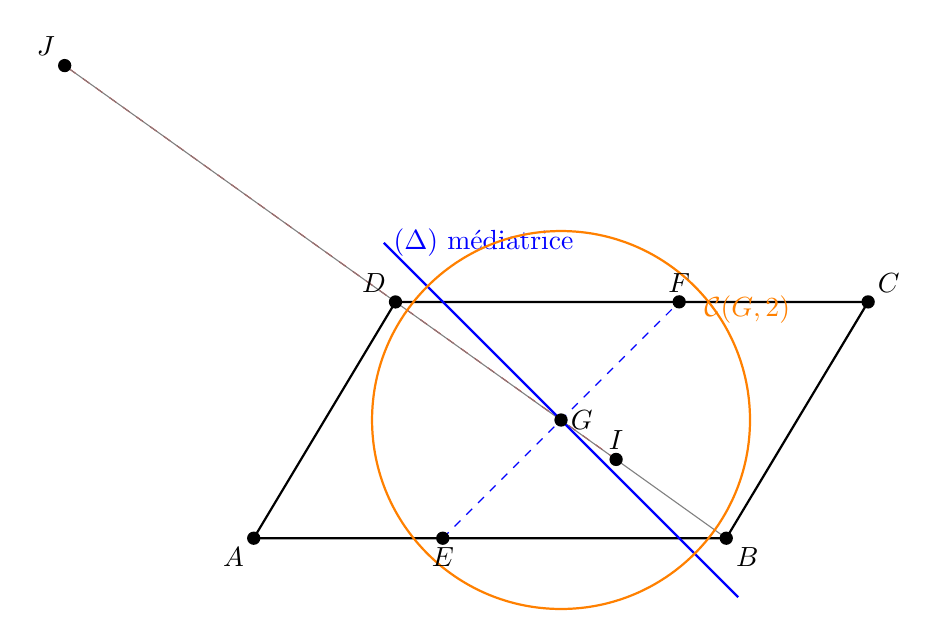
\begin{tikzpicture}[scale=1.2]
    % --- Définition des sommets du parallélogramme ABCD ---
    \coordinate (A) at (0,0);
    \coordinate (B) at (5,0);
    \coordinate (D) at (1.5,2.5);
    \coordinate (C) at ($(B)+(D)-(A)$); % Propriété du parallélogramme

    % --- Tracé du parallélogramme ---
    \draw[thick] (A) -- (B) -- (C) -- (D) -- cycle;

    % --- Question 1 : Points E et F ---
    % E = bar{(A,3);(B,2)} => AE = 2/5 AB
    \coordinate (E) at ($(A)!0.4!(B)$);
    % F = bar{(C,3);(D,2)} => CF = 2/5 CD
    \coordinate (F) at ($(C)!0.4!(D)$);

    % --- Question 2 : Point G (milieu de EF) ---
    \coordinate (G) at ($(E)!0.5!(F)$);

    % --- Question 3 : Points I et J ---
    % I = Centre de gravité de ABC = (A+B+C)/3
    \coordinate (I) at (barycentric cs:A=1,B=1,C=1);
    % J = symétrique de B par rapport à D => D milieu de BJ
    \coordinate (J) at ($(B)!2!(D)$);

    % --- Tracé des éléments de construction ---
    \draw[dashed, blue] (E) -- (F);
    \draw[dashed, red] (I) -- (J); % Droite d'alignement I, G, J
    \draw[gray, thin] (B) -- (J); % Segment pour J

    % --- Question 4 : Lieux géométriques ---
    % a) Médiatrice de [EF]
    \path (E) -- (F) node[midway, sloped] (midEF) {};
    \draw[blue, thick] ($(G)!1.5!90:(F)$) -- ($(G)!1.5!-90:(F)$);
    \node[blue, right] at ($(G)!1.5!90:(F)$) {($\Delta$) médiatrice};

    % b) Cercle de centre G et de rayon 2
    \draw[orange, thick] (G) circle (2cm);
    \node[orange, below right] at ($(G)+(45:2)$) {$\mathcal{C}(G, 2)$};

    % --- Affichage des points et labels ---
    \foreach \p/\pos in {A/below left, B/below right, C/above right, D/above left, E/below, F/above, G/right, I/above, J/above left}
        \fill (\p) circle (2pt) node[\pos] {$\p$};

\end{tikzpicture}
\end{center}

\section*{\underline{Correction – Exercice 2 :} Fonctions réelles}

\begin{enumerate}

%------------------------------------------------
\item \textbf{Détermination des domaines de définition}

\begin{enumerate}

%-------------------------
\item $f(x)=\dfrac{\sqrt{25-x^2}}{x-1}$

Pour que $f(x)$ soit définie :
\[
\begin{cases}
25-x^2 \ge 0 \\
x-1 \neq 0
\end{cases}
\]

La première condition donne :
\[
-5 \le x \le 5.
\]

La seconde condition impose :
\[
x \neq 1.
\]

\[
\boxed{D_f=[-5,5]\setminus\{1\}}
\]

%-------------------------
\item $f(x)=\sqrt{x^2-x+2}$

On doit avoir :
\[
x^2-x+2 \ge 0.
\]

Le discriminant vaut :
\[
\Delta=(-1)^2-4\times1\times2=-7<0.
\]

Donc $x^2-x+2>0$ pour tout $x\in\mathbb{R}$.

\[
\boxed{D_f=\mathbb{R}}
\]

%-------------------------
\item $f(x)=\dfrac{\sqrt{x^2-x-6}}{\sqrt{x^2-3x+2}}$

Conditions :
\[
\begin{cases}
x^2-x-6 \ge 0 \\
x^2-3x+2 > 0
\end{cases}
\]

On factorise :
\[
x^2-x-6=(x-3)(x+2),
\quad
x^2-3x+2=(x-1)(x-2).
\]

On obtient :
\[
(x-3)(x+2)\ge0
\quad \text{et} \quad
(x-1)(x-2)>0.
\]

Ainsi :
\[
\begin{aligned}
(x-3)(x+2)\ge0 &\Longleftrightarrow x\le -2 \ \text{ou}\ x\ge3,\\
(x-1)(x-2)>0 &\Longleftrightarrow x<1 \ \text{ou}\ x>2.
\end{aligned}
\]

Intersection :
\[
\boxed{D_f=]-\infty,-2]\cup[3,+\infty[}
\]

%-------------------------
\item 
\[
f(x)=
\begin{cases}
-x+\sqrt{x^2-x} & \text{si } x<0,\\[0.2cm]
\dfrac{x^3-5x}{x^2+3} & \text{si } x\ge0.
\end{cases}
\]

\begin{itemize}
\item Pour $x<0$, on exige :
\[
x^2-x \ge 0 \quad \Longleftrightarrow \quad x(x-1)\ge0.
\]
Ce qui donne $x\le0$ ou $x\ge1$.  
En tenant compte de $x<0$, on obtient $x<0$.

\item Pour $x\ge0$, le dénominateur $x^2+3>0$ pour tout $x$.
\end{itemize}

Donc :
\[
\boxed{D_f=\mathbb{R}}
\]

\end{enumerate}

%------------------------------------------------
\item \textbf{Soit $f(x)=\dfrac{4x^2+1}{2x^2+1}$ et $g(x)=3x-2$}

\begin{enumerate}

\item Calcul de $(g\circ f)(x)$

\[
(g\circ f)(x)=g\big(f(x)\big)
=3\left(\dfrac{4x^2+1}{2x^2+1}\right)-2.
\]

\[
(g\circ f)(x)
=\dfrac{12x^2+3-4x^2-2}{2x^2+1}
=\boxed{\dfrac{8x^2+1}{2x^2+1}}.
\]

\item Calcul de $(f\circ g)(x)$

\[
(f\circ g)(x)=f(3x-2)
=\dfrac{4(3x-2)^2+1}{2(3x-2)^2+1}.
\]

Or :
\[
(3x-2)^2=9x^2-12x+4.
\]

Ainsi :
\[
(f\circ g)(x)
=\boxed{\dfrac{36x^2-48x+17}{18x^2-24x+9}}.
\]

\end{enumerate}

%------------------------------------------------
\item \textbf{Soit $f(x)=|x+2|+|x-2|+2x$}

\begin{enumerate}

\item Expression de $f(x)$ sans valeur absolue \hfill \textbf{(0,75 pt)}

On étudie selon les valeurs de $x$ :

\[
\begin{cases}
x\le -2 : & f(x)=-(x+2)-(x-2)+2x=0,\\[0.2cm]
-2<x<2 : & f(x)=(x+2)-(x-2)+2x=2x+4,\\[0.2cm]
x\ge2 : & f(x)=(x+2)+(x-2)+2x=4x.
\end{cases}
\]

\item Restriction de $f$ à $]-\infty,-2]$ \hfill \textbf{(0,5 pt)}

Sur $]-\infty,-2]$, on a :
\[
\boxed{f(x)=0}.
\]

\end{enumerate}

\end{enumerate}

\section*{\underline{Correction – Exercice 3 :} Équations, inéquations et systèmes}

\begin{enumerate}

%--------------------------------------------------
\item \textbf{Résolution des équations et inéquations} \hfill \textbf{(0,75 pt $\times$ 4)}

\begin{enumerate}

%-------------------------
\item $\sqrt{2x-3}=x+2$

On doit avoir :
\[
\begin{cases}
2x-3 \ge 0 \\
x+2 \ge 0
\end{cases}
\quad \Longleftrightarrow \quad
x \ge \dfrac{3}{2}.
\]

On élève au carré :
\[
2x-3=(x+2)^2=x^2+4x+4.
\]

\[
x^2+2x+7=0.
\]

Le discriminant est :
\[
\Delta=2^2-4\times1\times7=-24<0.
\]

\[
\boxed{\text{Aucune solution réelle}}
\]

%-------------------------
\item $2x+\sqrt{x^2-4x-5}=18$

Condition :
\[
x^2-4x-5 \ge 0 \quad \Longleftrightarrow \quad x\le -1 \ \text{ou}\ x\ge5.
\]

On isole la racine :
\[
\sqrt{x^2-4x-5}=18-2x \quad \Rightarrow \quad 18-2x \ge 0 \Rightarrow x\le9.
\]

On élève au carré :
\[
x^2-4x-5=(18-2x)^2=4x^2-72x+324.
\]

\[
3x^2-68x+329=0.
\]

\[
\Delta=68^2-4\times3\times329=676.
\]

\[
x=\frac{68\pm26}{6} \Rightarrow x=7 \ \text{ou}\ x=\frac{47}{3}.
\]

Seul $x=7$ vérifie les conditions.

\[
\boxed{x=7}
\]

%-------------------------
\item $\sqrt{x-2} \le x-3$

Condition :
\[
x-2 \ge 0 \Rightarrow x \ge 2.
\]

Si $x-3<0$, l’inégalité est impossible car $\sqrt{x-2}\ge0$.

Donc :
\(
x-3 \ge 0 \Rightarrow x \ge 3.
\)

On élève au carré :
\[
x-2 \le (x-3)^2=x^2-6x+9.
\]

\[
x^2-7x+11 \ge 0.
\]

\[
\Delta=49-44=5.
\]

\[
x \le \frac{7-\sqrt5}{2} \quad \text{ou} \quad x \ge \frac{7+\sqrt5}{2}.
\]

En tenant compte de $x\ge3$ :
\[
\boxed{x \ge \dfrac{7+\sqrt5}{2}}
\]

%-------------------------
\item $\sqrt{x^2-x+1} \ge 2-x$

On remarque que :
\[
x^2-x+1>0 \quad \text{pour tout } x\in\mathbb{R}.
\]

\begin{itemize}
\item Si $2-x \le 0$ (i.e. $x\ge2$), l’inégalité est toujours vraie.
\item Si $x<2$, on élève au carré :
\[
x^2-x+1 \ge (2-x)^2=x^2-4x+4.
\]
\[
3x \ge 3 \Rightarrow x \ge 1.
\]
\end{itemize}

\[
\boxed{D=[1,+\infty[}
\]

\end{enumerate}

%--------------------------------------------------
\item \textbf{Détermination d’un polynôme du second degré} \hfill \textbf{(1,5 pt)}

Soit $f(x)=ax^2+bx+c$.

\[
\begin{cases}
a+b+c=0 \\
4a-2b+c=-3 \\
9a+3b+c=22
\end{cases}
\]

Soustraction :
\[
\begin{cases}
3a-3b=-3 \\
8a+2b=22
\end{cases}
\]

\[
a=2,\quad b=3,\quad c=-5.
\]

\[
\boxed{f(x)=2x^2+3x-5}
\]

%--------------------------------------------------
\item \textbf{Systèmes d’équations}

\begin{enumerate}

%-------------------------
\item Résolution par la méthode du pivot de Gauss \hfill \textbf{(1,5 pt)}

\[
\begin{cases}
x+2y+z=11 \\
2x+y-z=1 \\
4x-3y+z=7
\end{cases}
\]

\begin{comment}

Matrice augmentée :
\[
\left(
\begin{array}{ccc|c}
1 & 2 & 1 & 11 \\
2 & 1 & -1 & 1 \\
4 & -3 & 1 & 7
\end{array}
\right)
\]

Après opérations élémentaires :
\[
\left(
\begin{array}{ccc|c}
1 & 0 & 0 & 2 \\
0 & 1 & 0 & 3 \\
0 & 0 & 1 & 1
\end{array}
\right)
\]

\end{comment}

\[
\boxed{(x,y,z)=(2,3,1)}
\]

%-------------------------
\item Résolution des systèmes $(S)$ et $(S')$ \hfill \textbf{(1,5 pt)}

\textbf{Système $(S)$}

On pose :
\[
X=\frac{1}{x+3},\quad Y=\frac{1}{y+2},\quad Z=\frac{1}{z}.
\]

On retrouve le système précédent, donc :
\[
X=2,\ Y=3,\ Z=1.
\]

\[
\boxed{
\begin{cases}
x=-\dfrac{5}{2} \\
y=-\dfrac{5}{3} \\
z=1
\end{cases}}
\]

\textbf{Système $(S')$}

On pose :
\[
X=|x|,\quad Y=y^2,\quad Z=\frac{1}{z}.
\]

Même système, donc :
\[
|x|=2,\quad y^2=3,\quad z=1.
\]

\[
\boxed{
\begin{cases}
x=\pm2 \\
y=\pm\sqrt3 \\
z=1
\end{cases}}
\]

\end{enumerate}

\end{enumerate}

\section*{\underline{Correction – Exercice 4 :} Équations du second degré à paramètre}

\begin{enumerate}

%------------------------------------------------
\item \textbf{Soit l’équation $(E):\; x^2-(2m+1)x+m^2-2=0$}

\begin{enumerate}

%-------------------------
\item \textbf{Discussion selon les valeurs de $m$} \hfill \textbf{(1,5 pt)}

On calcule le discriminant :
\[
\Delta=(2m+1)^2-4(m^2-2).
\]

\[
\Delta=4m^2+4m+1-4m^2+8=4m+9.
\]

\begin{itemize}
    \item Si $4m+9>0 \iff m>-\dfrac{9}{4}$, alors $(E)$ admet deux solutions réelles distinctes :
    \[
    x'=\frac{2m+1-\sqrt{4m+9}}{2},
    \quad
    x''=\frac{2m+1+\sqrt{4m+9}}{2}.
    \]

    \item Si $4m+9=0 \iff m=-\dfrac{9}{4}$, alors $(E)$ admet une solution réelle double :
    \[
    x=\frac{2m+1}{2}=-\frac{7}{4}.
    \]

    \item Si $4m+9<0 \iff m<-\dfrac{9}{4}$, alors $(E)$ n’admet aucune solution réelle.
\end{itemize}

%-------------------------
\item \textbf{Dans le cas où $(E)$ admet deux solutions $x'$ et $x''$}

On suppose donc :
\[
m>-\frac{9}{4}.
\]

Par les relations de Viète :
\[
\begin{cases}
x'+x''=2m+1,\\
x'x''=m^2-2.
\end{cases}
\]

%-------------------------
\begin{enumerate}

\item \textbf{Condition $x'^2+x''^2=35$} \hfill \textbf{(0,75 pt)}

On utilise l’identité :
\[
x'^2+x''^2=(x'+x'')^2-2x'x''.
\]

\[
x'^2+x''^2=(2m+1)^2-2(m^2-2).
\]

\[
x'^2+x''^2=4m^2+4m+1-2m^2+4=2m^2+4m+5.
\]

On impose :
\[
2m^2+4m+5=35.
\]

\[
2m^2+4m-30=0 \iff m^2+2m-15=0.
\]

\[
(m+5)(m-3)=0.
\]

\[
\boxed{m=-5 \;\text{ou}\; m=3}
\]

Or $m>- \dfrac{9}{4}$, donc :
\[
\boxed{m=3}
\]

%-------------------------
\item \textbf{Condition $|x'-x''|=5$} \hfill \textbf{(0,75 pt)}

On sait que :
\[
|x'-x''|=\frac{\sqrt{\Delta}}{|a|}=\sqrt{4m+9}.
\]

Donc :
\[
\sqrt{4m+9}=5.
\]

\[
4m+9=25 \Rightarrow 4m=16 \Rightarrow m=4.
\]

Comme $m>-\dfrac{9}{4}$, la valeur est admissible.

\[
\boxed{m=4}
\]

\end{enumerate}

\end{enumerate}

\end{enumerate}


\end{document}
